% Number 620
% UFPM CAPMG Algebra Units
% Graphs: F to a to delta v, varying F
% JG

% Watermark
\AddToShipoutPicture*{\BackgroundPic}

\addtocounter {ProbNum} {1}

\begin{floatingfigure}[r]{.54\textwidth}
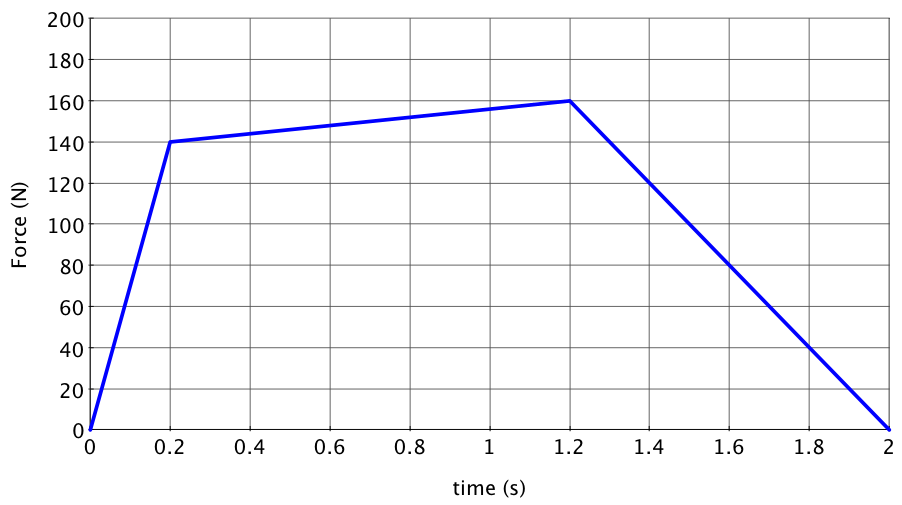
\includegraphics[scale=.7]{/Users/jgates/desktop/latex/pics/Fvst1}
\end{floatingfigure}
 
{\bf \Large{\arabic{ProbNum}}} A 50 kg peewee football player runs into a stationary 40 kg player at an initial speed of 4 meters per second. The magnitude of the force exerted by the football players on each other is shown as a function of time. 

\bigskip
Draw quantitatively accurate acceleration graphs for each player.
\paragraph{}
\noindent
\vfill
Use your acceleration graphs to determine the players' final velocities.
\vfill

Draw a motion diagram showing the players' motions before and after the collision.
\vspace{20mm}

%\hfill 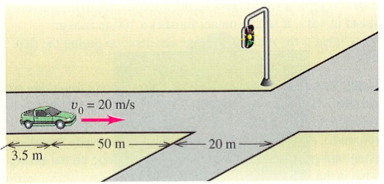
\includegraphics[scale=.85]{/Users/jgates/desktop/latex/pics/redlight.png}
\newpage